\documentclass[twoside]{book}

% Packages required by doxygen
\usepackage{fixltx2e}
\usepackage{calc}
\usepackage{doxygen}
\usepackage{graphicx}
\usepackage[utf8]{inputenc}
\usepackage{makeidx}
\usepackage{multicol}
\usepackage{multirow}
\PassOptionsToPackage{warn}{textcomp}
\usepackage{textcomp}
\usepackage[nointegrals]{wasysym}
\usepackage[table]{xcolor}

% Font selection
\usepackage[T1]{fontenc}
\usepackage{mathptmx}
\usepackage[scaled=.90]{helvet}
\usepackage{courier}
\usepackage{amssymb}
\usepackage{sectsty}
\renewcommand{\familydefault}{\sfdefault}
\allsectionsfont{%
  \fontseries{bc}\selectfont%
  \color{darkgray}%
}
\renewcommand{\DoxyLabelFont}{%
  \fontseries{bc}\selectfont%
  \color{darkgray}%
}
\newcommand{\+}{\discretionary{\mbox{\scriptsize$\hookleftarrow$}}{}{}}

% Page & text layout
\usepackage{geometry}
\geometry{%
  a4paper,%
  top=2.5cm,%
  bottom=2.5cm,%
  left=2.5cm,%
  right=2.5cm%
}
\tolerance=750
\hfuzz=15pt
\hbadness=750
\setlength{\emergencystretch}{15pt}
\setlength{\parindent}{0cm}
\setlength{\parskip}{0.2cm}
\makeatletter
\renewcommand{\paragraph}{%
  \@startsection{paragraph}{4}{0ex}{-1.0ex}{1.0ex}{%
    \normalfont\normalsize\bfseries\SS@parafont%
  }%
}
\renewcommand{\subparagraph}{%
  \@startsection{subparagraph}{5}{0ex}{-1.0ex}{1.0ex}{%
    \normalfont\normalsize\bfseries\SS@subparafont%
  }%
}
\makeatother

% Headers & footers
\usepackage{fancyhdr}
\pagestyle{fancyplain}
\fancyhead[LE]{\fancyplain{}{\bfseries\thepage}}
\fancyhead[CE]{\fancyplain{}{}}
\fancyhead[RE]{\fancyplain{}{\bfseries\leftmark}}
\fancyhead[LO]{\fancyplain{}{\bfseries\rightmark}}
\fancyhead[CO]{\fancyplain{}{}}
\fancyhead[RO]{\fancyplain{}{\bfseries\thepage}}
\fancyfoot[LE]{\fancyplain{}{}}
\fancyfoot[CE]{\fancyplain{}{}}
\fancyfoot[RE]{\fancyplain{}{\bfseries\scriptsize Generated on Sat Oct 11 2014 07\+:13\+:44 for Sound Editor by Doxygen }}
\fancyfoot[LO]{\fancyplain{}{\bfseries\scriptsize Generated on Sat Oct 11 2014 07\+:13\+:44 for Sound Editor by Doxygen }}
\fancyfoot[CO]{\fancyplain{}{}}
\fancyfoot[RO]{\fancyplain{}{}}
\renewcommand{\footrulewidth}{0.4pt}
\renewcommand{\chaptermark}[1]{%
  \markboth{#1}{}%
}
\renewcommand{\sectionmark}[1]{%
  \markright{\thesection\ #1}%
}

% Indices & bibliography
\usepackage{natbib}
\usepackage[titles]{tocloft}
\setcounter{tocdepth}{3}
\setcounter{secnumdepth}{5}
\makeindex

% Hyperlinks (required, but should be loaded last)
\usepackage{ifpdf}
\ifpdf
  \usepackage[pdftex,pagebackref=true]{hyperref}
\else
  \usepackage[ps2pdf,pagebackref=true]{hyperref}
\fi
\hypersetup{%
  colorlinks=true,%
  linkcolor=blue,%
  citecolor=blue,%
  unicode%
}

% Custom commands
\newcommand{\clearemptydoublepage}{%
  \newpage{\pagestyle{empty}\cleardoublepage}%
}


%===== C O N T E N T S =====

\begin{document}

% Titlepage & ToC
\hypersetup{pageanchor=false,
             bookmarks=true,
             bookmarksnumbered=true,
             pdfencoding=unicode
            }
\pagenumbering{roman}
\begin{titlepage}
\vspace*{7cm}
\begin{center}%
{\Large Sound Editor }\\
\vspace*{1cm}
{\large Generated by Doxygen 1.8.8}\\
\vspace*{0.5cm}
{\small Sat Oct 11 2014 07:13:44}\\
\end{center}
\end{titlepage}
\clearemptydoublepage
\tableofcontents
\clearemptydoublepage
\pagenumbering{arabic}
\hypersetup{pageanchor=true}

%--- Begin generated contents ---
\chapter{Hierarchical Index}
\section{Class Hierarchy}
This inheritance list is sorted roughly, but not completely, alphabetically\-:\begin{DoxyCompactList}
\item $<$A\-V\-Audio\-Player\-Delegate$>$\begin{DoxyCompactList}
\item \contentsline{section}{S\-E\-Sound()}{\pageref{category_s_e_sound_07_08}}{}
\end{DoxyCompactList}
\item $<$A\-V\-Audio\-Recorder\-Delegate$>$\begin{DoxyCompactList}
\item \contentsline{section}{S\-E\-Sound()}{\pageref{category_s_e_sound_07_08}}{}
\end{DoxyCompactList}
\item N\-S\-Object\begin{DoxyCompactList}
\item \contentsline{section}{S\-E\-Audio\-Stream}{\pageref{interface_s_e_audio_stream}}{}
\item \contentsline{section}{S\-E\-Audio\-Stream\-Player}{\pageref{interface_s_e_audio_stream_player}}{}
\item \contentsline{section}{S\-E\-Sound}{\pageref{interface_s_e_sound}}{}
\item \contentsline{section}{S\-R\-Audio\-Stream\-Player}{\pageref{interface_s_r_audio_stream_player}}{}
\end{DoxyCompactList}
\item $<$N\-S\-Object\-N\-S\-Object$>$\begin{DoxyCompactList}
\item \contentsline{section}{$<$S\-E\-Audio\-Stream\-Player\-Delegate$>$}{\pageref{protocol_s_e_audio_stream_player_delegate-p}}{}
\item \contentsline{section}{$<$S\-R\-Audio\-Stream\-Delegate$>$}{\pageref{protocol_s_r_audio_stream_delegate-p}}{}
\item \contentsline{section}{$<$S\-R\-Sound\-Delegate$>$}{\pageref{protocol_s_r_sound_delegate-p}}{}
\end{DoxyCompactList}
\item \contentsline{section}{S\-E\-Audio\-Stream(Read)}{\pageref{category_s_e_audio_stream_07_read_08}}{}
\item \contentsline{section}{S\-E\-Audio\-Stream(Write)}{\pageref{category_s_e_audio_stream_07_write_08}}{}
\item \contentsline{section}{S\-E\-Project()}{\pageref{category_s_e_project_07_08}}{}
\item \contentsline{section}{S\-R\-Audio\-Stream\-Player()}{\pageref{category_s_r_audio_stream_player_07_08}}{}
\item S\-R\-Model\begin{DoxyCompactList}
\item \contentsline{section}{S\-E\-Project}{\pageref{interface_s_e_project}}{}
\item \contentsline{section}{S\-E\-Record}{\pageref{interface_s_e_record}}{}
\end{DoxyCompactList}
\item \contentsline{section}{S\-R\-Sound\-Range}{\pageref{struct_s_r_sound_range}}{}
\end{DoxyCompactList}

\chapter{Class Index}
\section{Class List}
Here are the classes, structs, unions and interfaces with brief descriptions\-:\begin{DoxyCompactList}
\item\contentsline{section}{\hyperlink{class_application_u_i}{Application\-U\-I} \\*Application object }{\pageref{class_application_u_i}}{}
\end{DoxyCompactList}

\chapter{Class Documentation}
\hypertarget{class_s_e_audio_stream}{\section{S\+E\+Audio\+Stream Class Reference}
\label{class_s_e_audio_stream}\index{S\+E\+Audio\+Stream@{S\+E\+Audio\+Stream}}
}
Inheritance diagram for S\+E\+Audio\+Stream\+:\begin{figure}[H]
\begin{center}
\leavevmode
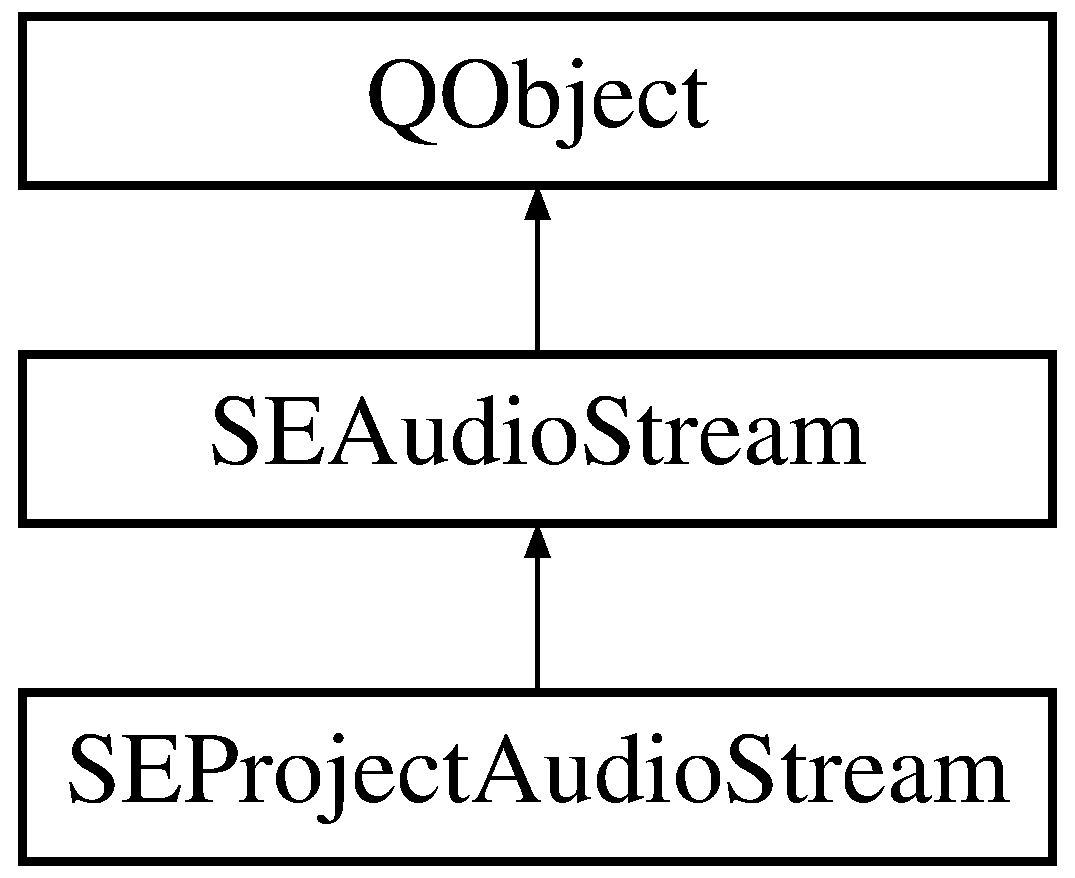
\includegraphics[height=3.000000cm]{class_s_e_audio_stream}
\end{center}
\end{figure}
\subsection*{Public Member Functions}
\begin{DoxyCompactItemize}
\item 
\hypertarget{class_s_e_audio_stream_ad4400267e4d64428f82f5b774e64d89d}{{\bfseries S\+E\+Audio\+Stream} (Q\+String path, Q\+Object $\ast$parent=0)}\label{class_s_e_audio_stream_ad4400267e4d64428f82f5b774e64d89d}

\item 
\hypertarget{class_s_e_audio_stream_acb2cd924f6e33ef742f30a750e0708f3}{Q\+String {\bfseries get\+Path} ()}\label{class_s_e_audio_stream_acb2cd924f6e33ef742f30a750e0708f3}

\item 
\hypertarget{class_s_e_audio_stream_a64f1a25545197281d9f556e9371511e2}{virtual long {\bfseries get\+Duration} ()}\label{class_s_e_audio_stream_a64f1a25545197281d9f556e9371511e2}

\item 
\hypertarget{class_s_e_audio_stream_a73cbe0d712b86dac39028cd0967474f3}{virtual void {\bfseries set\+Description} (\hyperlink{struct_t_s_e_audio_stream_desc}{T\+S\+E\+Audio\+Stream\+Desc} desc)}\label{class_s_e_audio_stream_a73cbe0d712b86dac39028cd0967474f3}

\item 
\hypertarget{class_s_e_audio_stream_af6cb98f0366c35353b6e6c7b2d0ffe24}{\hyperlink{struct_t_s_e_audio_stream_desc}{T\+S\+E\+Audio\+Stream\+Desc} {\bfseries get\+Description} ()}\label{class_s_e_audio_stream_af6cb98f0366c35353b6e6c7b2d0ffe24}

\item 
\hypertarget{class_s_e_audio_stream_ac1234e9c052d73def9f6a8b71516ec01}{T\+S\+E\+Audio\+Stream\+Mode {\bfseries get\+Mode} ()}\label{class_s_e_audio_stream_ac1234e9c052d73def9f6a8b71516ec01}

\item 
\hypertarget{class_s_e_audio_stream_a270d3f5b03562d1284fbe74060a6b32e}{virtual bool {\bfseries open} (T\+S\+E\+Audio\+Stream\+Mode mode)}\label{class_s_e_audio_stream_a270d3f5b03562d1284fbe74060a6b32e}

\item 
\hypertarget{class_s_e_audio_stream_a8c4af367964e8be4817df12989f06d40}{virtual void {\bfseries close} ()}\label{class_s_e_audio_stream_a8c4af367964e8be4817df12989f06d40}

\item 
\hypertarget{class_s_e_audio_stream_ab9c31f1004bbdf45ec8caee753ee127e}{virtual bool {\bfseries read\+Data} (Q\+Byte\+Array \&byte\+Array, long position, long duration)}\label{class_s_e_audio_stream_ab9c31f1004bbdf45ec8caee753ee127e}

\item 
\hypertarget{class_s_e_audio_stream_aecda3096d9dca88eca934a2a555ad0ff}{virtual bool {\bfseries write\+Data} (Q\+Byte\+Array \&byte\+Array)}\label{class_s_e_audio_stream_aecda3096d9dca88eca934a2a555ad0ff}

\item 
\hypertarget{class_s_e_audio_stream_ae8d33acef5174c832e229c61d1c5d75d}{bool {\bfseries export\+To\+Audio\+Stream} (\hyperlink{class_s_e_audio_stream}{S\+E\+Audio\+Stream} $\ast$audio\+Stream)}\label{class_s_e_audio_stream_ae8d33acef5174c832e229c61d1c5d75d}

\end{DoxyCompactItemize}
\subsection*{Protected Member Functions}
\begin{DoxyCompactItemize}
\item 
\hypertarget{class_s_e_audio_stream_a9e6533e1ca6a98463a208a6a668b0fcc}{void {\bfseries reload\+Desc} ()}\label{class_s_e_audio_stream_a9e6533e1ca6a98463a208a6a668b0fcc}

\end{DoxyCompactItemize}
\subsection*{Protected Attributes}
\begin{DoxyCompactItemize}
\item 
\hypertarget{class_s_e_audio_stream_aa0b683207a891441919b456b52ecc9af}{Q\+String {\bfseries path}}\label{class_s_e_audio_stream_aa0b683207a891441919b456b52ecc9af}

\item 
\hypertarget{class_s_e_audio_stream_afde89d08f02ae01b1e9be3905942fb31}{T\+S\+E\+Audio\+Stream\+Mode {\bfseries mode}}\label{class_s_e_audio_stream_afde89d08f02ae01b1e9be3905942fb31}

\item 
\hypertarget{class_s_e_audio_stream_a0c7455be26d6addadbeed52c78cf1d68}{Wave\+File $\ast$ {\bfseries file}}\label{class_s_e_audio_stream_a0c7455be26d6addadbeed52c78cf1d68}

\item 
\hypertarget{class_s_e_audio_stream_a689abf52d876db852fa8c28c3fbaec12}{\hyperlink{struct_t_s_e_audio_stream_desc}{T\+S\+E\+Audio\+Stream\+Desc} {\bfseries desc}}\label{class_s_e_audio_stream_a689abf52d876db852fa8c28c3fbaec12}

\end{DoxyCompactItemize}


The documentation for this class was generated from the following files\+:\begin{DoxyCompactItemize}
\item 
/\+Users/igor/\+Develop/\+Devacon/\+Blackberry/\+Sound\+Editor/src/\+Core/S\+E\+Audio\+Stream.\+h\item 
/\+Users/igor/\+Develop/\+Devacon/\+Blackberry/\+Sound\+Editor/src/\+Core/S\+E\+Audio\+Stream.\+cpp\end{DoxyCompactItemize}

\hypertarget{class_s_e_audio_stream_engine}{\section{S\+E\+Audio\+Stream\+Engine Class Reference}
\label{class_s_e_audio_stream_engine}\index{S\+E\+Audio\+Stream\+Engine@{S\+E\+Audio\+Stream\+Engine}}
}
Inheritance diagram for S\+E\+Audio\+Stream\+Engine\+:\begin{figure}[H]
\begin{center}
\leavevmode
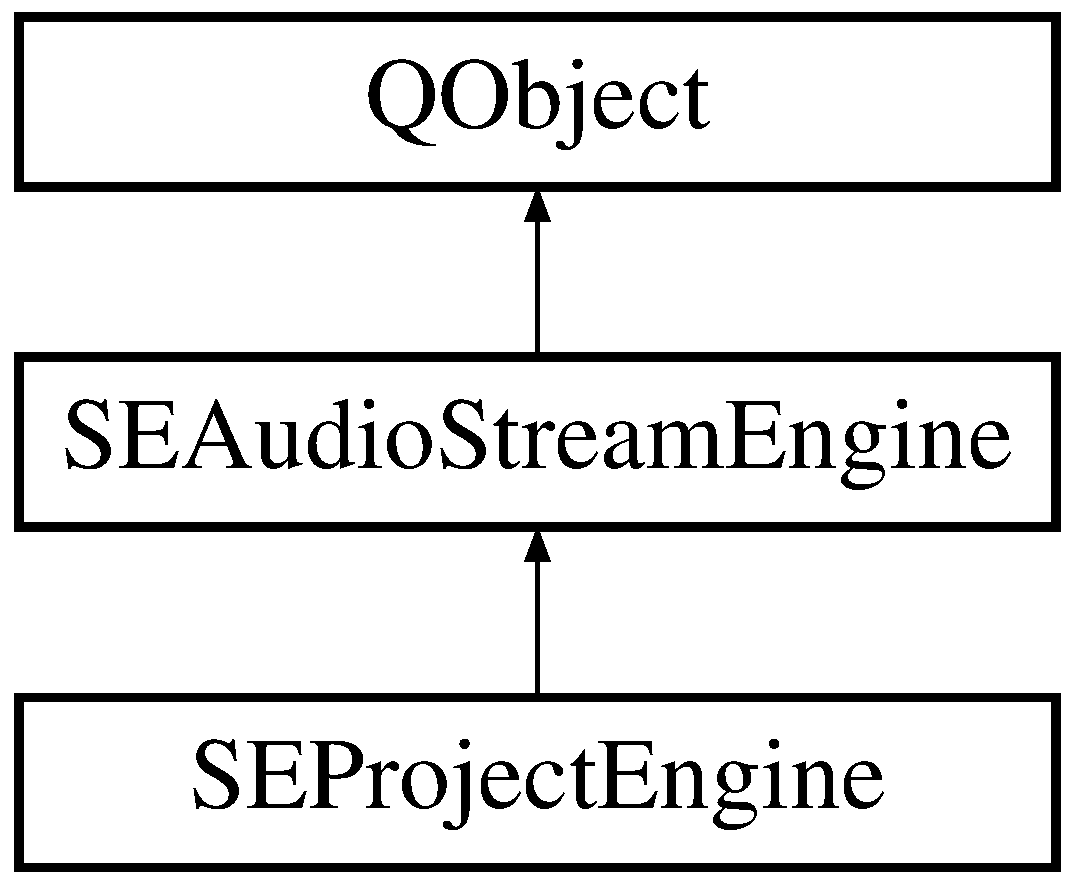
\includegraphics[height=3.000000cm]{class_s_e_audio_stream_engine}
\end{center}
\end{figure}
\subsection*{Signals}
\begin{DoxyCompactItemize}
\item 
\hypertarget{class_s_e_audio_stream_engine_a6e3666a25828115786cc39ad40741a9d}{void {\bfseries start\+Playing} ()}\label{class_s_e_audio_stream_engine_a6e3666a25828115786cc39ad40741a9d}

\item 
\hypertarget{class_s_e_audio_stream_engine_ae75c4a24cb45b92433a0f954c7180489}{void {\bfseries pause\+Playing} ()}\label{class_s_e_audio_stream_engine_ae75c4a24cb45b92433a0f954c7180489}

\item 
\hypertarget{class_s_e_audio_stream_engine_a0b15249dddcd7d84668dcd1e36c556a1}{void {\bfseries continue\+Playing} ()}\label{class_s_e_audio_stream_engine_a0b15249dddcd7d84668dcd1e36c556a1}

\item 
\hypertarget{class_s_e_audio_stream_engine_a10a870faaaa71521fe1455d938b2d789}{void {\bfseries update\+Playing} (double time)}\label{class_s_e_audio_stream_engine_a10a870faaaa71521fe1455d938b2d789}

\item 
\hypertarget{class_s_e_audio_stream_engine_a77d1d55cf373ab32b01d20b7997b13f2}{void {\bfseries stop\+Playing} ()}\label{class_s_e_audio_stream_engine_a77d1d55cf373ab32b01d20b7997b13f2}

\item 
\hypertarget{class_s_e_audio_stream_engine_ad19a0488b4ea40ae9ae54c38526895de}{void {\bfseries start\+Recording} ()}\label{class_s_e_audio_stream_engine_ad19a0488b4ea40ae9ae54c38526895de}

\item 
\hypertarget{class_s_e_audio_stream_engine_aa42610b8261e058f34fbebb7b51d5e3a}{void {\bfseries update\+Recording} (double time)}\label{class_s_e_audio_stream_engine_aa42610b8261e058f34fbebb7b51d5e3a}

\item 
\hypertarget{class_s_e_audio_stream_engine_a2a1cd707ceb8fb2801826c38d932da66}{void {\bfseries stop\+Recording} ()}\label{class_s_e_audio_stream_engine_a2a1cd707ceb8fb2801826c38d932da66}

\item 
\hypertarget{class_s_e_audio_stream_engine_a5aab9b32d7a76483925c9a5365f806de}{void {\bfseries error\+Occurred} (Q\+String error)}\label{class_s_e_audio_stream_engine_a5aab9b32d7a76483925c9a5365f806de}

\end{DoxyCompactItemize}
\subsection*{Public Member Functions}
\begin{DoxyCompactItemize}
\item 
\hypertarget{class_s_e_audio_stream_engine_aa09fbccd738ff9c5da7dc892725ff0af}{{\bfseries S\+E\+Audio\+Stream\+Engine} (\hyperlink{class_s_e_audio_stream}{S\+E\+Audio\+Stream} $\ast$stream, Q\+Object $\ast$parent=0)}\label{class_s_e_audio_stream_engine_aa09fbccd738ff9c5da7dc892725ff0af}

\item 
\hypertarget{class_s_e_audio_stream_engine_a6b35e0ac97d167b2116e282607571bad}{T\+S\+E\+Audio\+Stream\+Engine\+State {\bfseries get\+State} ()}\label{class_s_e_audio_stream_engine_a6b35e0ac97d167b2116e282607571bad}

\item 
\hypertarget{class_s_e_audio_stream_engine_a2b339016ae6c29cc904228fd44ee01c6}{double {\bfseries get\+Duration} ()}\label{class_s_e_audio_stream_engine_a2b339016ae6c29cc904228fd44ee01c6}

\item 
\hypertarget{class_s_e_audio_stream_engine_a150f918934337e35e3d905441edf49e8}{void {\bfseries set\+Current\+Position} (double position)}\label{class_s_e_audio_stream_engine_a150f918934337e35e3d905441edf49e8}

\item 
\hypertarget{class_s_e_audio_stream_engine_a74e52f79b260973168c93a4bd8cfc9ce}{double {\bfseries get\+Current\+Position} ()}\label{class_s_e_audio_stream_engine_a74e52f79b260973168c93a4bd8cfc9ce}

\item 
\hypertarget{class_s_e_audio_stream_engine_aba880904dacd4ff95a6689fcd0517cf7}{\hyperlink{class_s_e_audio_stream}{S\+E\+Audio\+Stream} $\ast$ {\bfseries get\+Stream} ()}\label{class_s_e_audio_stream_engine_aba880904dacd4ff95a6689fcd0517cf7}

\item 
\hypertarget{class_s_e_audio_stream_engine_a216867458e22624b0ac08ffa98c5fa31}{void {\bfseries play} ()}\label{class_s_e_audio_stream_engine_a216867458e22624b0ac08ffa98c5fa31}

\item 
\hypertarget{class_s_e_audio_stream_engine_adf3e9101e926e949a2d3d79642810592}{void {\bfseries pause} ()}\label{class_s_e_audio_stream_engine_adf3e9101e926e949a2d3d79642810592}

\item 
\hypertarget{class_s_e_audio_stream_engine_acdfd6d3c3ff61a0c62efacbea6648158}{void {\bfseries record} ()}\label{class_s_e_audio_stream_engine_acdfd6d3c3ff61a0c62efacbea6648158}

\item 
\hypertarget{class_s_e_audio_stream_engine_a4e03579a7199bd59954a9a30b37805c4}{void {\bfseries stop} ()}\label{class_s_e_audio_stream_engine_a4e03579a7199bd59954a9a30b37805c4}

\end{DoxyCompactItemize}
\subsection*{Protected Attributes}
\begin{DoxyCompactItemize}
\item 
\hypertarget{class_s_e_audio_stream_engine_a686e9ac0b8133e2da5e5aac566fe312e}{\hyperlink{class_s_e_audio_stream}{S\+E\+Audio\+Stream} $\ast$ {\bfseries stream}}\label{class_s_e_audio_stream_engine_a686e9ac0b8133e2da5e5aac566fe312e}

\item 
\hypertarget{class_s_e_audio_stream_engine_a33e4a362e1da557272aee227935da239}{S\+E\+Audio\+Stream\+Player $\ast$ {\bfseries player}}\label{class_s_e_audio_stream_engine_a33e4a362e1da557272aee227935da239}

\item 
\hypertarget{class_s_e_audio_stream_engine_ac492313c93cee8d5ca05fc5001a4afdc}{S\+E\+Audio\+Stream\+Recorder $\ast$ {\bfseries recorder}}\label{class_s_e_audio_stream_engine_ac492313c93cee8d5ca05fc5001a4afdc}

\item 
\hypertarget{class_s_e_audio_stream_engine_a124d47656b0b46ef4ec62ead90d17c47}{T\+S\+E\+Audio\+Stream\+Engine\+State {\bfseries state}}\label{class_s_e_audio_stream_engine_a124d47656b0b46ef4ec62ead90d17c47}

\item 
\hypertarget{class_s_e_audio_stream_engine_a3899ff2022b38cd5a0dc132a53ba417f}{long {\bfseries position}}\label{class_s_e_audio_stream_engine_a3899ff2022b38cd5a0dc132a53ba417f}

\end{DoxyCompactItemize}


The documentation for this class was generated from the following files\+:\begin{DoxyCompactItemize}
\item 
/\+Users/igor/\+Develop/\+Devacon/\+Blackberry/\+Sound\+Editor/src/\+Core/S\+E\+Audio\+Stream\+Engine.\+h\item 
/\+Users/igor/\+Develop/\+Devacon/\+Blackberry/\+Sound\+Editor/src/\+Core/S\+E\+Audio\+Stream\+Engine.\+cpp\end{DoxyCompactItemize}

\hypertarget{class_s_e_project}{\section{S\+E\+Project Class Reference}
\label{class_s_e_project}\index{S\+E\+Project@{S\+E\+Project}}
}
Inheritance diagram for S\+E\+Project\+:\begin{figure}[H]
\begin{center}
\leavevmode
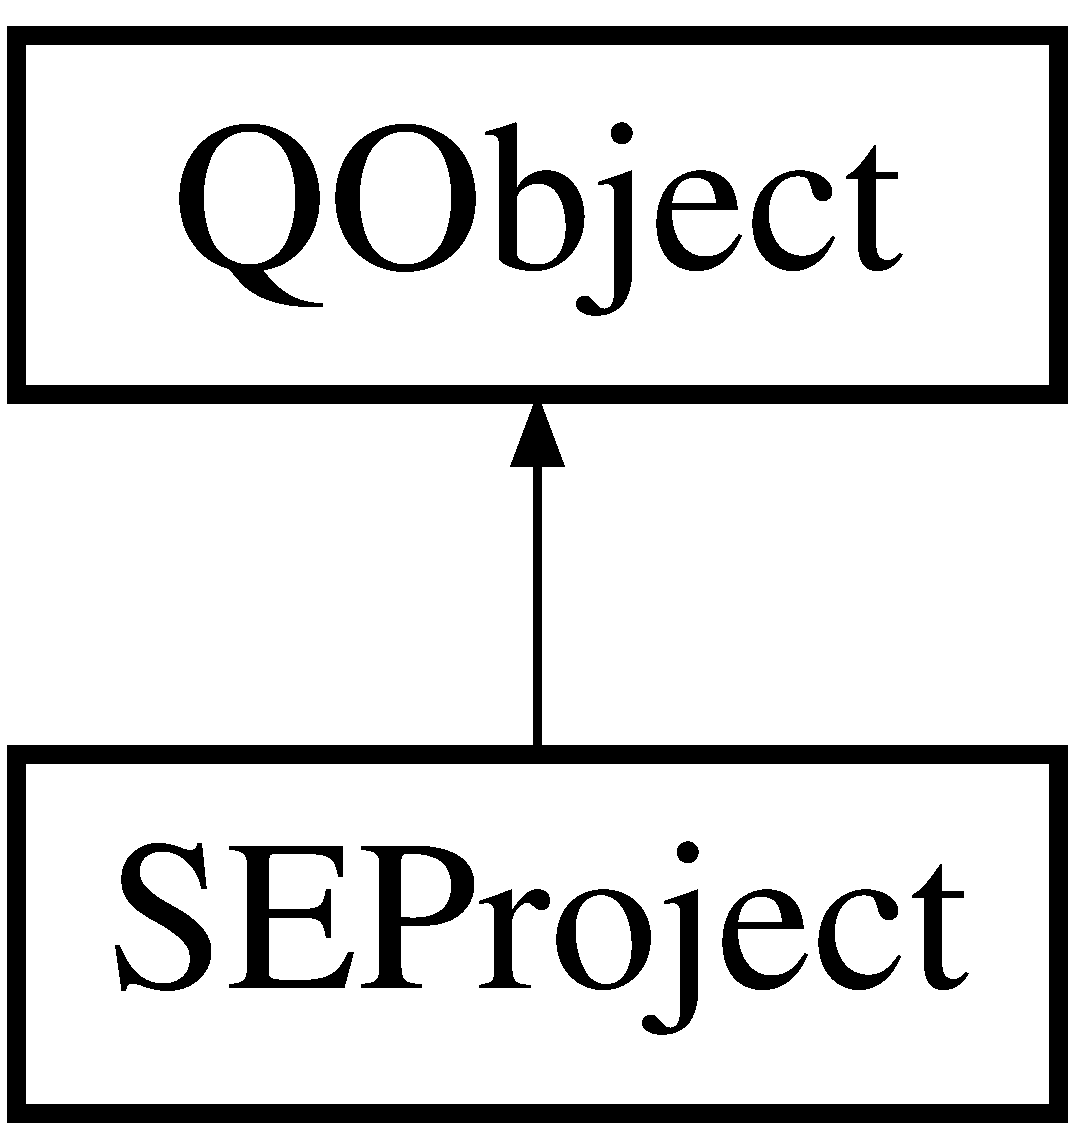
\includegraphics[height=2.000000cm]{class_s_e_project}
\end{center}
\end{figure}
\subsection*{Public Member Functions}
\begin{DoxyCompactItemize}
\item 
\hypertarget{class_s_e_project_ac2f839342520e02740af686e3d067703}{{\bfseries S\+E\+Project} (Q\+String project\+Folder\+Name, Q\+Object $\ast$parent=0)}\label{class_s_e_project_ac2f839342520e02740af686e3d067703}

\item 
\hypertarget{class_s_e_project_a7b42ff1cf09ed8c7a0ae70b6df5c1654}{\hyperlink{class_s_e_audio_stream}{S\+E\+Audio\+Stream} $\ast$ {\bfseries get\+Audio\+Stream} ()}\label{class_s_e_project_a7b42ff1cf09ed8c7a0ae70b6df5c1654}

\item 
\hypertarget{class_s_e_project_a0ab936035b3df3bd82bf6f28488e9bab}{void {\bfseries set\+Name} (Q\+String name)}\label{class_s_e_project_a0ab936035b3df3bd82bf6f28488e9bab}

\item 
\hypertarget{class_s_e_project_ad2d4c5ac6dc7aaacdabf94ce20408def}{Q\+String {\bfseries get\+Name} ()}\label{class_s_e_project_ad2d4c5ac6dc7aaacdabf94ce20408def}

\item 
\hypertarget{class_s_e_project_acb93acf37e7efad3abf19eb157146037}{Q\+String {\bfseries get\+Project\+Path} ()}\label{class_s_e_project_acb93acf37e7efad3abf19eb157146037}

\item 
\hypertarget{class_s_e_project_a073414bd0ed96671a8ed55722c4136a2}{Q\+String {\bfseries get\+Project\+Sound\+Path} ()}\label{class_s_e_project_a073414bd0ed96671a8ed55722c4136a2}

\item 
\hypertarget{class_s_e_project_a191586c8f8464149aa101709b3b712b9}{void {\bfseries clear\+Project} ()}\label{class_s_e_project_a191586c8f8464149aa101709b3b712b9}

\item 
\hypertarget{class_s_e_project_ad0dc83a89c70e8a670d2e0eb0381e632}{void {\bfseries save\+Project} ()}\label{class_s_e_project_ad0dc83a89c70e8a670d2e0eb0381e632}

\item 
\hypertarget{class_s_e_project_ae52dee786ff60fa56ec078a45db79293}{void {\bfseries add\+Record} (S\+E\+Record $\ast$record)}\label{class_s_e_project_ae52dee786ff60fa56ec078a45db79293}

\item 
\hypertarget{class_s_e_project_a960cb8f84ef856c84ed27da15adb3eeb}{void {\bfseries remove\+Record} (S\+E\+Record $\ast$record)}\label{class_s_e_project_a960cb8f84ef856c84ed27da15adb3eeb}

\item 
\hypertarget{class_s_e_project_ad509d4afbd0a2ce3973c92179fe31eec}{void {\bfseries insert\+Record} (S\+E\+Record $\ast$record, int index)}\label{class_s_e_project_ad509d4afbd0a2ce3973c92179fe31eec}

\item 
\hypertarget{class_s_e_project_a3d61ce7fe9afeed0a461d47232498148}{S\+E\+Record $\ast$ {\bfseries split\+Record\+In\+Position} (long position)}\label{class_s_e_project_a3d61ce7fe9afeed0a461d47232498148}

\item 
\hypertarget{class_s_e_project_a27d4de382ffc61d9b92235704a554ebd}{Q\+List$<$ S\+E\+Record $\ast$ $>$ {\bfseries get\+Records} ()}\label{class_s_e_project_a27d4de382ffc61d9b92235704a554ebd}

\end{DoxyCompactItemize}


The documentation for this class was generated from the following files\+:\begin{DoxyCompactItemize}
\item 
/\+Users/igor/\+Develop/\+Devacon/\+Blackberry/\+Sound\+Editor/src/\+Core/S\+E\+Project.\+h\item 
/\+Users/igor/\+Develop/\+Devacon/\+Blackberry/\+Sound\+Editor/src/\+Core/S\+E\+Project.\+cpp\end{DoxyCompactItemize}

\hypertarget{class_s_e_project_audio_stream}{\section{S\+E\+Project\+Audio\+Stream Class Reference}
\label{class_s_e_project_audio_stream}\index{S\+E\+Project\+Audio\+Stream@{S\+E\+Project\+Audio\+Stream}}
}
Inheritance diagram for S\+E\+Project\+Audio\+Stream\+:\begin{figure}[H]
\begin{center}
\leavevmode
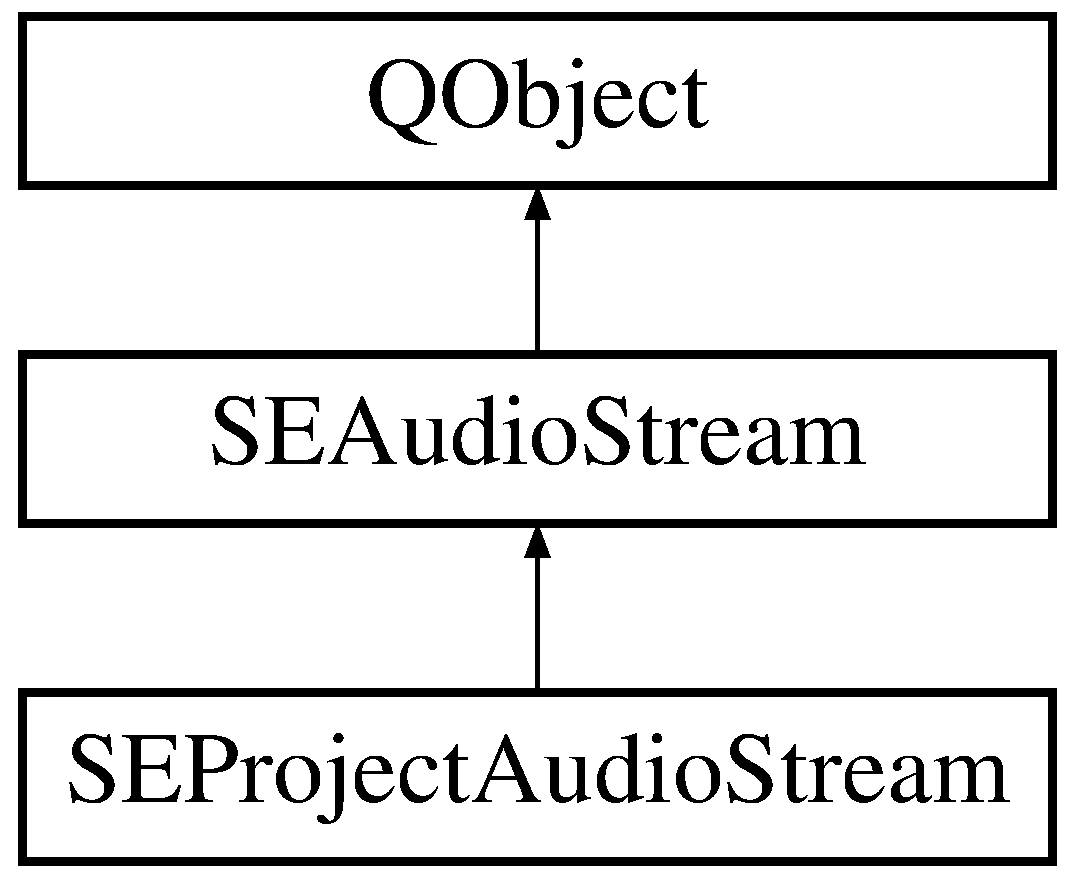
\includegraphics[height=3.000000cm]{class_s_e_project_audio_stream}
\end{center}
\end{figure}
\subsection*{Public Member Functions}
\begin{DoxyCompactItemize}
\item 
\hypertarget{class_s_e_project_audio_stream_ac653618185dafa5f040cadfc76c281fa}{{\bfseries S\+E\+Project\+Audio\+Stream} (\hyperlink{class_s_e_project}{S\+E\+Project} $\ast$project, Q\+Object $\ast$parent=0)}\label{class_s_e_project_audio_stream_ac653618185dafa5f040cadfc76c281fa}

\item 
\hypertarget{class_s_e_project_audio_stream_ad59f3e75ba6d28b6fdf35a7b56671118}{long {\bfseries get\+Duration} ()}\label{class_s_e_project_audio_stream_ad59f3e75ba6d28b6fdf35a7b56671118}

\item 
\hypertarget{class_s_e_project_audio_stream_adf20fdc6fe02c955dd512180c27018af}{bool {\bfseries read\+Data} (Q\+Byte\+Array \&byte\+Array, long position, long duration)}\label{class_s_e_project_audio_stream_adf20fdc6fe02c955dd512180c27018af}

\item 
\hypertarget{class_s_e_project_audio_stream_a2c89f777534b37424972e34cea3d0fe6}{bool {\bfseries open} (T\+S\+E\+Audio\+Stream\+Mode mode)}\label{class_s_e_project_audio_stream_a2c89f777534b37424972e34cea3d0fe6}

\item 
\hypertarget{class_s_e_project_audio_stream_a738f8d4e0313042b798a3caa0fe59ca0}{void {\bfseries close} ()}\label{class_s_e_project_audio_stream_a738f8d4e0313042b798a3caa0fe59ca0}

\end{DoxyCompactItemize}
\subsection*{Additional Inherited Members}


The documentation for this class was generated from the following files\+:\begin{DoxyCompactItemize}
\item 
/\+Users/igor/\+Develop/\+Devacon/\+Blackberry/\+Sound\+Editor/src/\+Core/S\+E\+Project\+Audio\+Stream.\+h\item 
/\+Users/igor/\+Develop/\+Devacon/\+Blackberry/\+Sound\+Editor/src/\+Core/S\+E\+Project\+Audio\+Stream.\+cpp\end{DoxyCompactItemize}

\hypertarget{class_s_e_project_engine}{\section{S\+E\+Project\+Engine Class Reference}
\label{class_s_e_project_engine}\index{S\+E\+Project\+Engine@{S\+E\+Project\+Engine}}
}
Inheritance diagram for S\+E\+Project\+Engine\+:\begin{figure}[H]
\begin{center}
\leavevmode
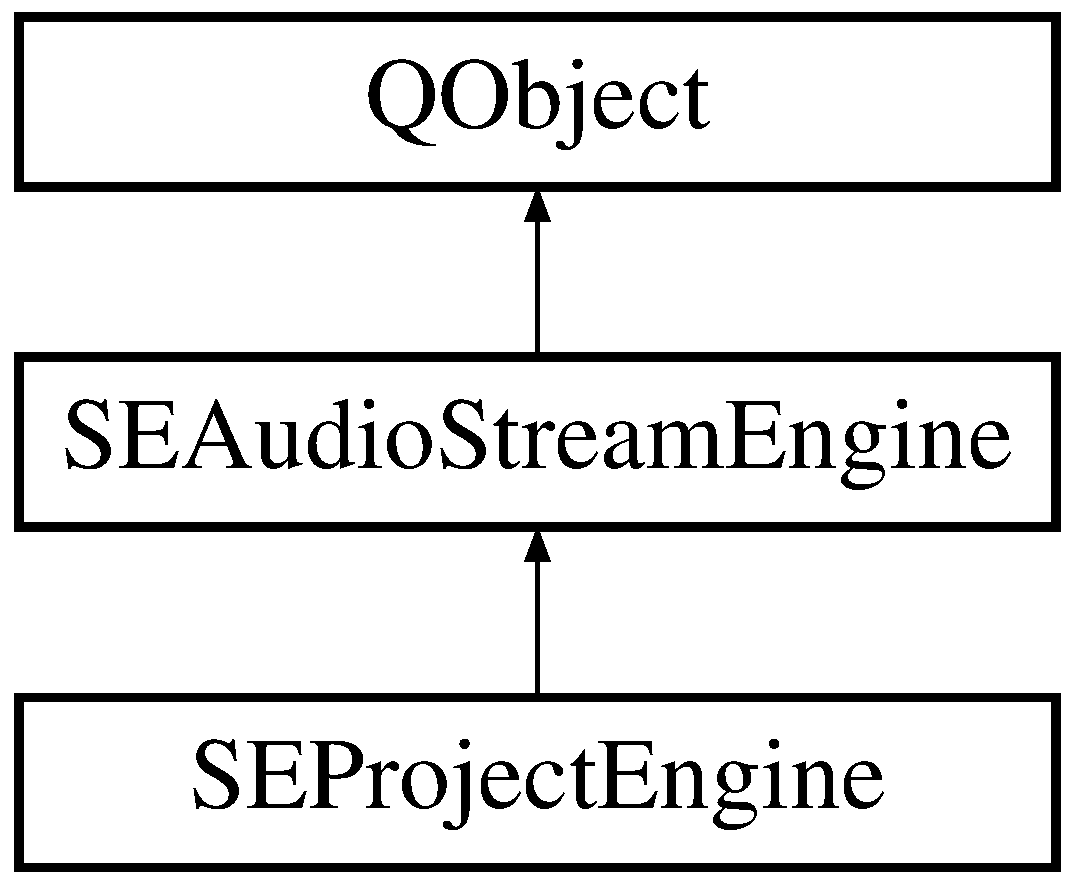
\includegraphics[height=3.000000cm]{class_s_e_project_engine}
\end{center}
\end{figure}
\subsection*{Public Member Functions}
\begin{DoxyCompactItemize}
\item 
\hypertarget{class_s_e_project_engine_abb5f13a09c01fe607dddde31da5e4fd1}{{\bfseries S\+E\+Project\+Engine} (\hyperlink{class_s_e_project}{S\+E\+Project} $\ast$project, Q\+Object $\ast$parent=0)}\label{class_s_e_project_engine_abb5f13a09c01fe607dddde31da5e4fd1}

\item 
\hypertarget{class_s_e_project_engine_a878e47d3eae756f4f8521a49d18dcca2}{double {\bfseries get\+Duration} ()}\label{class_s_e_project_engine_a878e47d3eae756f4f8521a49d18dcca2}

\item 
\hypertarget{class_s_e_project_engine_adf72e62511341059690d59af562fbb0f}{void {\bfseries record} ()}\label{class_s_e_project_engine_adf72e62511341059690d59af562fbb0f}

\item 
\hypertarget{class_s_e_project_engine_ab5d875c023cf7e083b1a7c90b1d9b622}{void {\bfseries stop} ()}\label{class_s_e_project_engine_ab5d875c023cf7e083b1a7c90b1d9b622}

\item 
\hypertarget{class_s_e_project_engine_aaae1596505f3ec4550cf7b7e6f40960f}{void {\bfseries clear} ()}\label{class_s_e_project_engine_aaae1596505f3ec4550cf7b7e6f40960f}

\end{DoxyCompactItemize}
\subsection*{Additional Inherited Members}


The documentation for this class was generated from the following files\+:\begin{DoxyCompactItemize}
\item 
/\+Users/igor/\+Develop/\+Devacon/\+Blackberry/\+Sound\+Editor/src/\+Core/S\+E\+Project\+Engine.\+h\item 
/\+Users/igor/\+Develop/\+Devacon/\+Blackberry/\+Sound\+Editor/src/\+Core/S\+E\+Project\+Engine.\+cpp\end{DoxyCompactItemize}

\hypertarget{struct_t_s_e_audio_stream_desc}{\section{T\+S\+E\+Audio\+Stream\+Desc Struct Reference}
\label{struct_t_s_e_audio_stream_desc}\index{T\+S\+E\+Audio\+Stream\+Desc@{T\+S\+E\+Audio\+Stream\+Desc}}
}
\subsection*{Public Attributes}
\begin{DoxyCompactItemize}
\item 
\hypertarget{struct_t_s_e_audio_stream_desc_a445b2e676e52f5a895210747cb799dde}{unsigned short {\bfseries audio\+Format}}\label{struct_t_s_e_audio_stream_desc_a445b2e676e52f5a895210747cb799dde}

\item 
\hypertarget{struct_t_s_e_audio_stream_desc_ae7893c4aaf66e0d9042bfda1ad602a21}{unsigned short {\bfseries number\+Of\+Channels}}\label{struct_t_s_e_audio_stream_desc_ae7893c4aaf66e0d9042bfda1ad602a21}

\item 
\hypertarget{struct_t_s_e_audio_stream_desc_a1088958be0c2d74002d679794ee4b334}{unsigned long {\bfseries sample\+Rate}}\label{struct_t_s_e_audio_stream_desc_a1088958be0c2d74002d679794ee4b334}

\item 
\hypertarget{struct_t_s_e_audio_stream_desc_ad90671d7b383c097807fd016938ff592}{unsigned long {\bfseries bytes\+Per\+Second}}\label{struct_t_s_e_audio_stream_desc_ad90671d7b383c097807fd016938ff592}

\item 
\hypertarget{struct_t_s_e_audio_stream_desc_ab9cc22ba2bca64941688daf573486d4f}{unsigned short {\bfseries bytes\+Per\+Sample}}\label{struct_t_s_e_audio_stream_desc_ab9cc22ba2bca64941688daf573486d4f}

\item 
\hypertarget{struct_t_s_e_audio_stream_desc_a4ea25ab0e18b87816731c4b4eab40b52}{unsigned short {\bfseries bits\+Per\+Sample}}\label{struct_t_s_e_audio_stream_desc_a4ea25ab0e18b87816731c4b4eab40b52}

\end{DoxyCompactItemize}


The documentation for this struct was generated from the following file\+:\begin{DoxyCompactItemize}
\item 
/\+Users/igor/\+Develop/\+Devacon/\+Blackberry/\+Sound\+Editor/src/\+Core/S\+E\+Audio\+Stream.\+h\end{DoxyCompactItemize}

%--- End generated contents ---

% Index
\newpage
\phantomsection
\addcontentsline{toc}{chapter}{Index}
\printindex

\end{document}
